\section{Numerical Experiments}

We now provide numerical evidence of the efficiency of our method. All the  experiments have been carried out  with Tensorflow 2.7  on a 2021 Macbook pro with 64GB unified memory and Apple M1 Max chip. The code is implemented in Python and run on CPU (10-core) only.  
Throughout the examples, we use the same neural network architecture and training parameters,  given  below:
\begin{enumerate}
\item The feedforward neural network consists of $2$ hidden layers, each having $20 + \text{dim}(\calE)$  nodes  with leaky rectified linear unit (Leaky ReLU) activation function. The output layer uses the standard rectified linear unit (ReLU)  activation. Moreover, the  bias in the output layer, say $\theta_0 \in \R$, can be used to set  an initial threshold level. From our observations, the algorithm is not sensitive to $\theta_0$, as long as it is set to a reasonable value.  For fixed strike payoffs of the form  $\eqref{eq:payoff}$, we  choose $\theta_0=\frac{3K}{2}$,  $\theta_0=\frac{K}{2}$ for  calls 
and puts
,  respectively.

%  In other words, the  threshold function reads
% $$G(t,\xi; \theta) = \left(\theta_0 + \theta_1^{\top} G_{-1}(t,\xi; \theta_{-1})\right)^+, \quad (\theta_{-1}, \theta_{0}, \theta_1) = \theta, $$ %, \quad \theta_1 \in \R^{50+\bar{d}}
% where  $G_{-1}(t,\xi; \theta_{-1}) \in \R^{20+\bar{d}}$ is the value of the neural network before entering the output layer.



\item The number of training iterations is set to $M=3,000$ and batch size to $B = 512$. 
    \item The learning rates $(\zeta_m)$ are obtained from the widely accepted Adam optimizer \cite{Kingma}.
    
    \item  
    If the payoff function is of the form
    $\eqref{eq:payoff}$ (which is the case in all the examples below), the fuzzy boundary width is chosen to be    
    $\epsilon_n = K \sqrt{\V^{\Q}[ \alpha(X^{t_{n-1},1}_{t_n})]}$, $t_n \in \calT_N$. 
     The strike $K$ takes account the scale of the payoff$-$and in turn, the threshold function$-$while  the second in $\epsilon_n$ reflects the typical variation 
     of the  process $\alpha(X)$ between exercise dates. When the exercise dates are equally spaced, we simply write $\epsilon$ instead of $\epsilon_n$. 
\end{enumerate}
Once the training phase is completed,  we compute the initial price using the sharp boundary and $J= 2^{22} = 4,194,304$ Monte Carlo simulations. 

\subsection{Put Option in the Black-Scholes Model} \label{sec:putBS}
Consider an ATM Bermudan put option ($\varphi(s) = (K-s)^+$) in the Black Scholes model. We take the same parameters as in  Section 4.3.1.2 of \cite{Becker2}, namely
$S_0=K=40$, $r = 6\%$, $\delta = 0\%$, $\sigma = 40\%$, with maturity $T=1$ and exercise dates $\calT_{\!N} = \{\frac{n}{N} \ | \ n=0,\ldots,N\}$, $N=50$.  
As the stock price must reach low values to cross the boundary, we can use importance sampling to make the drift of $S-$which is positive under $\Q-$negative under an equivalent measure. We can for instance set $\lambda \equiv \frac{r-\delta + 0.05}{\sigma}  = 0.275$ so $S$ becomes a submartingale under $\Q^{\lambda}$ with $5\%$ negative drift. Notice that the fuzzy boundary width is approximately equal to $\epsilon = K\sigma \sqrt{T/N}$.  \cref{tab:resultPutBS} summarizes the result, in comparison with the value found by \citet{Becker1}. The first column is the average price of ten experiments and the second column the highest price. In practice, we would of course retain the trained boundary yielding the highest price. 

\begin{table}[ht]
  \centering
  \caption{Bermudan Put Option ($N=50$), Black-Scholes model.  
 }
 
 \vspace{-2mm}
 
  \begin{tabular}{cccc}
 \hline \hline
    Average Price  & Highest Price & Runtime  & Price in \cite{Becker2}  \\
  \hline  \hline
  5.308 (0.003)  &  5.313 (0.003) &  57.9 & 5.311 \\
  \hline \\[-1em]
  
  \multicolumn{4}{l}{%
  \begin{minipage}{9.cm}%
    \tiny \textit{First  column:  average  of ten experiments (standard deviation in brackets). Second column: highest price  among the realisations and its standard deviation in brackets.  Third column:  average runtime (in seconds) per experiment for the training phase.}%
  \end{minipage}%
}

\end{tabular}
\vspace{2mm}
% \begin{flushleft}
% \scriptsize{
% \textit{Notes:  }}
% \end{flushleft}
\label{tab:resultPutBS}
  \end{table}

Figure \ref{fig:putBS} displays the initial boundary (left chart) with the trained one (right chart) compared with the optimal boundary. The latter is obtained using a finite-difference scheme.  

\begin{figure}
    \centering
    \caption{Exercise boundary (Bermudan put,  Black-Scholes model).}
    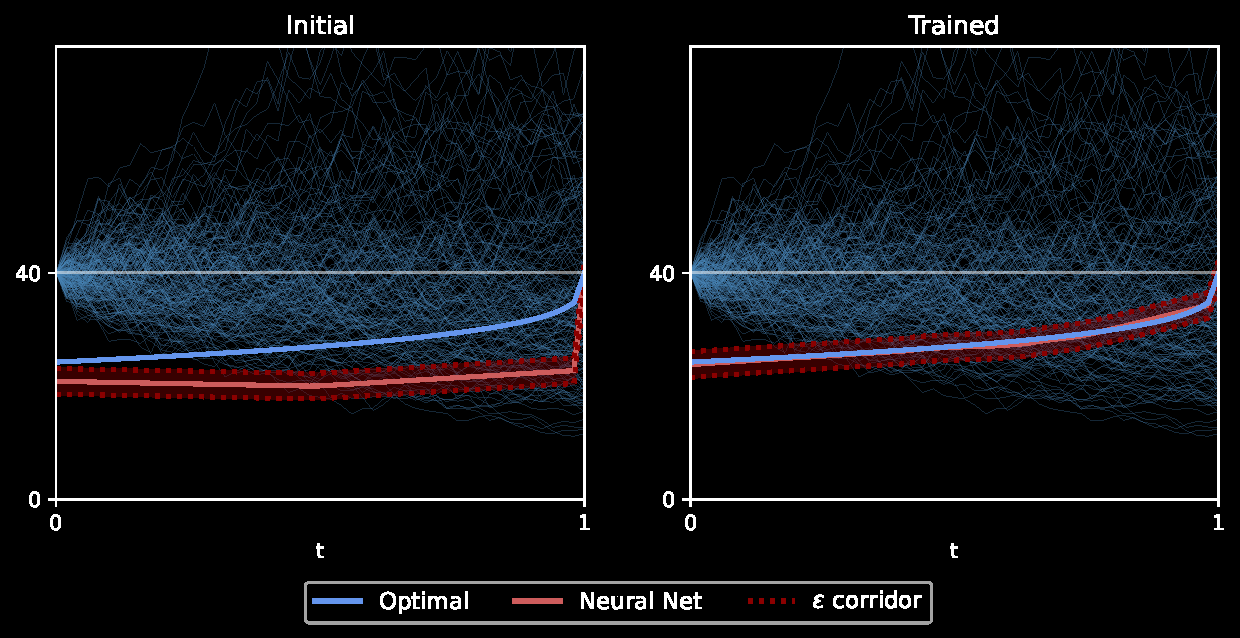
\includegraphics[scale=0.5]{Figures/Bdry 2, lbda=0.275, mu=0.050, N=50.pdf}
    
    \label{fig:putBS}
\end{figure}

\subsection{Put Option in the Heston Model}\label{sec:putHeston}

Consider the Bermudan put option from the previous section ($S_0 =K=40$, $T=1$, $N=50$) in the Heston model. Our goal is to see how stochastic volatility impacts the exercise boundary and  corresponding  price.   
 Let $m=1, \ k=0$ and assume the stock and factor dynamics
\begin{align}
   \frac{dS_t}{S_t} &= (r-\delta)dt + \sqrt{\calV_t}\  dW_t, \\
   d\calV_t &= (\kappa(\bar{\nu}-\calV_t) - \gamma^{\Q}\calV_t)dt + \sigma_{\calV} \sqrt{\calV_t}\  d\tilde{W}_t, \label{eq:varSDE}
\end{align}
with $\calV_0 = \nu_0 \in \R^2_+$ and $\frac{d\langle W, \tilde{W} \rangle_t}{dt} = \rho  \in  (-1,1)$. 
We choose the parameters
 $r = 6\%$, $\delta = 0\%$, $\kappa = 1$, $\nu_0 = \bar{\nu} = (40\%)^2$, $\gamma^{\Q} =0$, $\sigma_{\calV} =10\%$, and $\rho =-0.5$. In particular, 
the Feller condition $\kappa \,  \bar{\nu} \ge  \frac{\sigma_{\calV}^2}{2}$ is satisfied.  
For a fair comparison,  we set the initial value and long term mean of $\calV$ equal to the Black-Scholes variance $\sigma^2$ from \cref{sec:putBS}.   Moreover, we use importance sampling with same Girsanov parameter, i.e. $\lambda \equiv \frac{r-\delta + 0.05}{\sigma}  = 0.275$. The  variance process is simulated using the Milstein-Platen scheme \cite{KP} for $\eqref{eq:varSDE}$ with $N' =4N=200$ time steps.  %on a thinner partition $\Pi_{N'}$ with $N' =200$. 

As seen in \cref{ex:vanilla}, the threshold function 
depends on time $t$ and the spot variance $\calV_t =\nu$.  
When $\varphi$ is convex and bounded (which is the case here)   \citet{LambertonHeston} showed that the value function $v(t,x)$, $x=(s,\nu)$, is  non-decreasing in $\nu$ for all $t\in [0,T]$. Consequently, the map $\nu \mapsto f(t,\nu)$ is non-increasing. As can be seen in  \cref{fig:heston1}, it turns out that the same holds for the trained neural network $G(\cdot,\cdot;\theta^M)$.
Notice also that $\nu \mapsto f(t,\nu)$ becomes less steep as $t$ approaches maturity. This is line with the fact that the Vega  decreases over time until the option is exercised.  
As $s \to v(t,s,\nu)$ is non-increasing for fixed $(t,\nu)$,  we therefore expect that the  rectangle $[0,s]\times [0,\nu]$ 
is contained in $\calS_t$ whenever $(s,\nu) \in \calS_t$. This is confirmed in  \cref{fig:heston1}. 

 
\begin{figure}[H]
    \centering
     \caption{Stopping and continuation regions (Bermudan put, Heston model).}
    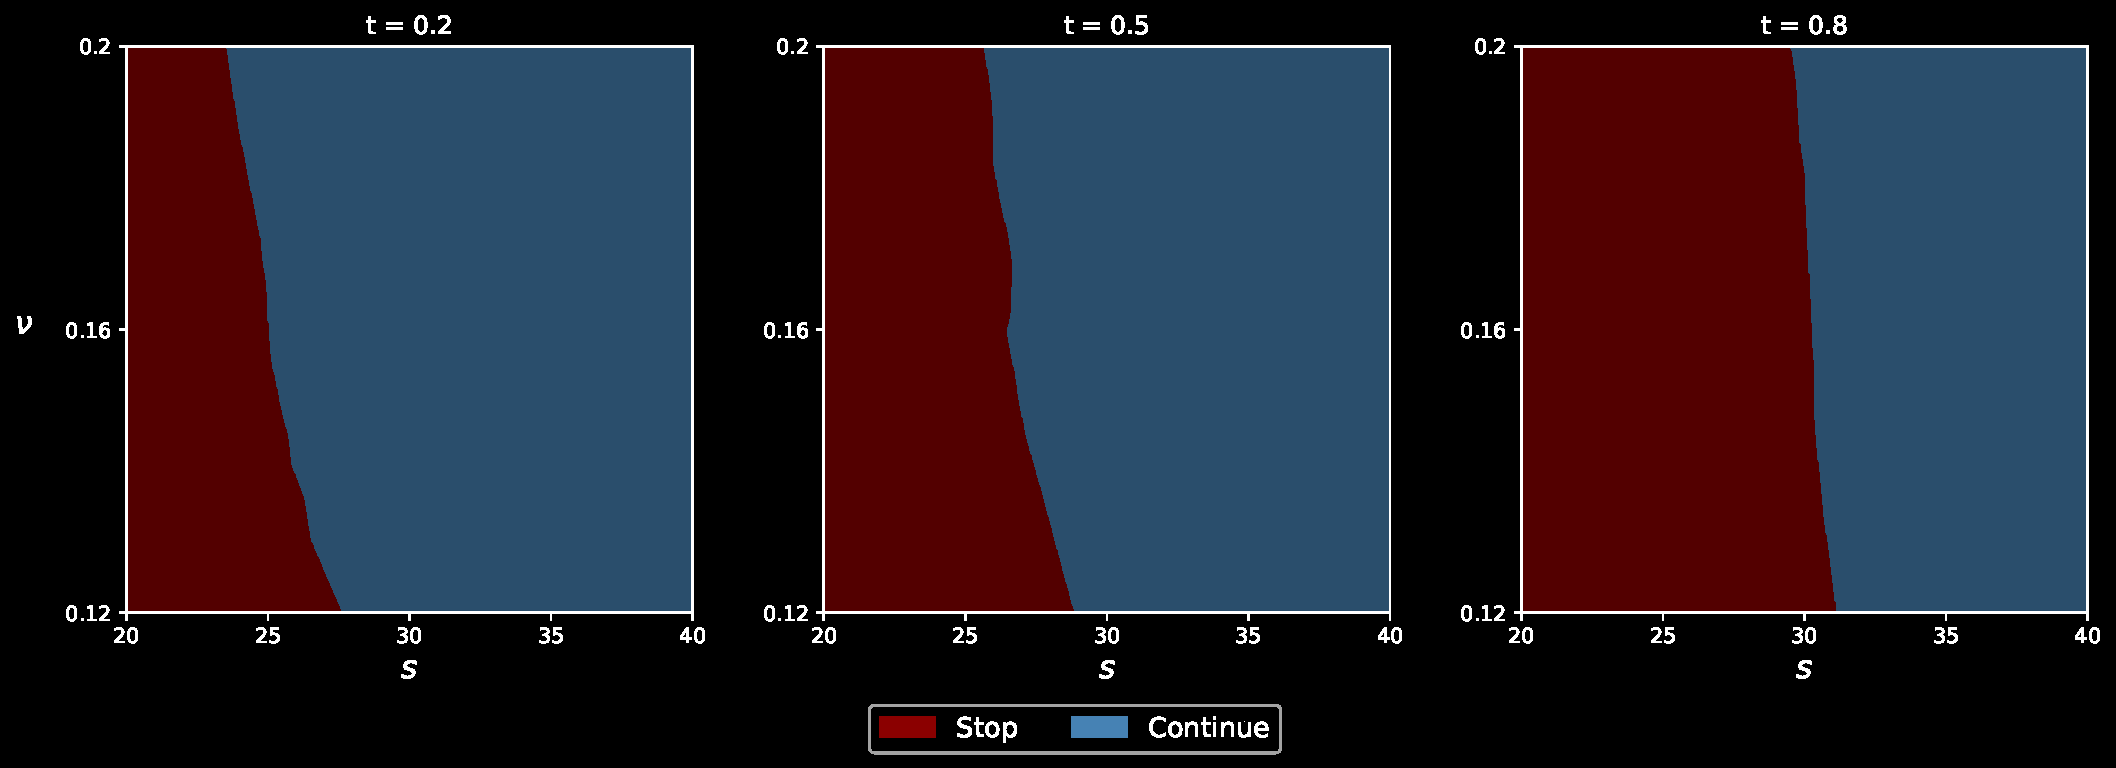
\includegraphics[scale = 0.42]{Figures/2DPlotHestonWide.pdf}
    \label{fig:heston1}
\end{figure}

 \cref{tab:resultPutHeston} compares the price of the claim when the stopping decision exploit the spot variance ($f = f(t,\nu)$) and when it does not ($f = f(t)$). We observe that the price obtained with the "blind" strategy is only slightly inferior. Interestingly, the neural network coincides with the optimal boundary in the Black-Scholes model.  Note also the longer runtime compared to \cref{tab:resultPutBS} due to the thin partition needed to simulate $\calV$. %, as shown in Figure \cref{fig:heston1}
 Finally, \cref{fig:heston2} displays a trajectory for $(X,\calV)$ together with the threshold process $G(\cdot,\calV;\theta^M)$. As can be seen, the threshold is typically below the Black-Scholes boundary when $\calV_t$ is above its mean $\bar{\nu} = 0.16$ and vice versa. 

\begin{table}[ht]
  \centering
  \caption{Bermudan Put Option ($N=50$), Heston model.}  
 
 \vspace{-2mm}
 
  \begin{tabular}{c c c c }
 \hline  \hline
  Threshold &  Average Price& Highest Price & Runtime  \\
  \hline  \hline
    $f(t,\nu)$ & 5.290 (0.004) & 5.294 (0.003) &  194.3 \\
  $f(t)$ & 5.288 (0.004) & 5.293 (0.003) &  193.9  \\
  \hline\\[-1em]
    
  \multicolumn{4}{l}{%
  \begin{minipage}{9.cm}%
    \tiny \textit{Second  column:  average  of ten experiments (standard deviation in brackets). Third column: highest price  among the realisations and its standard deviation in brackets.  Fourth column:  average runtime (in seconds) per experiment for the training phase.}%
  \end{minipage} }
\end{tabular}
\vspace{2mm}
\label{tab:resultPutHeston}
  \end{table}
 

\begin{figure}[H]
    \centering
     \caption{Stock price, variance and threshold process (Bermudan put, Heston model).}
    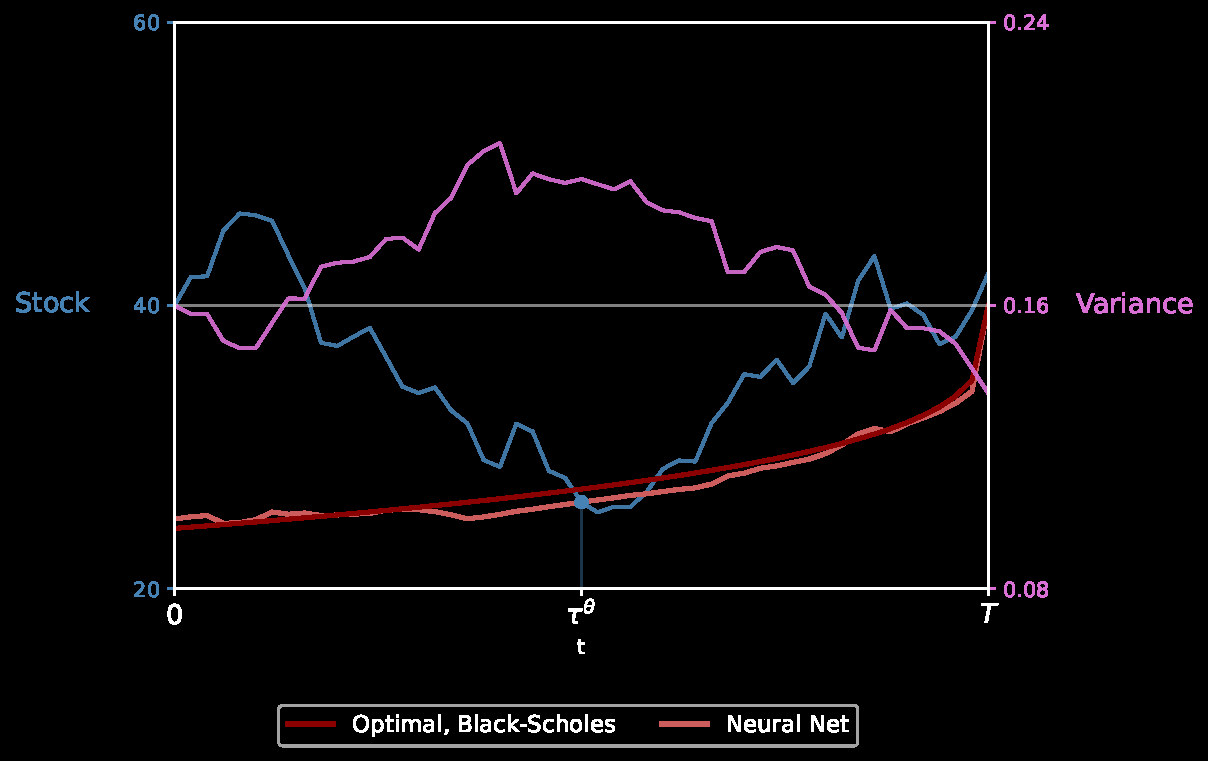
\includegraphics[scale = 0.4]{Figures/BdryHeston2.pdf}
    \label{fig:heston2}
\end{figure}


\subsection{High-dimensional Max Option on Symmetric Assets}\label{sec:maxCallSym}
Consider a Bermudan max option (see \cref{ex:max}) %($\alpha(s) = \max_{i=1,...,d}s_i$, $\beta\equiv 0$, $\eta=1$) 
with strike $K=100$, maturity $T=3$ and triannual exercise dates, i.e. $\calT_{\! N} = \{\frac{n}{3} \ | \ n=0,\ldots,N\}$, $N=9$.  Consider the multi-dimensional Black-Scholes model with independent and symmetric assets, i.e. 
\begin{align}\label{eq:multiBS}
    d S_t = \text{diag}(S_t) \left[ (r - \delta)\mathds{1} dt + \sigma dW_t\right],
\end{align}
where $W$ is Brownian motion in $\R^d$, $\mathds{1} = (1,\ldots,1) \in \R^d$, and $r,\delta,\sigma$ are nonnegative scalars. 
We employ the parameters from Section 4.4.1 in \cite{Becker2}, that is $s_0 =100 $, $r=5\%$, $\delta =10\%$ and $\sigma = 20 \%$. 

 First, notice that the drift of $\alpha(S_t) = \max_{i=1,...,d}S_{t,i}$  increases with $d$. More precisely, we observed that the additional drift is of order $\calO(\log d)$. To ensure that the maximum doesn't exceed the threshold function too soon, we use importance sampling with $\lambda_d = \frac{r-\delta + \mu_d}{\sigma}$, where $\mu_d = 0.01 \log d\ $ gives satisfactory results. % as we shall see below.  %\bb{Drift $\mu_d$}

As both the payoff and assets are symmetric, it is easily shown that  $\calS_t$ is symmetric as well; see \cref{sec:symmetry}. This property can be exploited to reduce the dimension of our problem. Indeed, observe that it suffices to characterize the $t-$sections of the stopping region in the \textit{cone of ordered stocks}  
 $\calO = \{s\in \R_+^d \,|\, s_1 \geq \ldots \geq s_d\}$. We can therefore arrange $\Xi(S_t) = \frac{S_t}{\alpha(S_t)}\in [0,1]^d$ in decreasing order and give the outcome to $G(t,\cdot; \theta)$. If $\bar{S}_t \in \calO$ denotes the ordered version of $S_t$, then the last components of $\bar{S}_t$ are of little relevance to our stopping decision. 
 Indeed, over a short horizon, the maximum stock value is likely to be attained by one of the current best performing assets. %a stock having a high value today. at the next exercise date
 We can therefore set a cutoff $2 \le d' \ll d$ and feed the neural network with $(\frac{\bar{S}_{t,2}}{\alpha(S_t)},\ldots,\frac{\bar{S}_{t,d'}}{\alpha(S_t)})$ only.\footnote{Note that $\frac{\bar{S}_{t,1}}{\alpha(S_t)} \equiv 1$ is also removed from the neural network input as it doesn't carry any information.} Although one still needs to simulate $d$ assets, the size of the neural network can be significantly reduced, which in turn accelerates the training phase. 
 
We compute the initial price of the max option on $d \in\{2,5,10,20,50\}$ assets with cutoff   $d'=5$.    
 \cref{tab:symMaxOpt} summarizes the results. Despite a low cutoff, the  obtained prices are close or above the benchmark.
 Moreover, the runtime remains moderate as $d$ increases. The case $d=5$ is a classical example first concocted by \citet{BroadieGlasserman} and well-studied in the literature. We added in  \cref{tab:symMaxOpt} the tight confidence interval obtained by \citet{BroadieCao} using a primal-dual method. As can be seen, our average price lies between the lower and upper bound.

\begin{table}[ht]
\caption{Max Option on $d \in\{5,10,20,50\}$ symmetric assets}

\vspace{-2mm}
\label{tab:symMaxOpt}
  \centering
  \begin{tabular}{ c c c c c c}
 \hline  \hline
   $d$ & Average Price& Highest Price & Runtime& Price in \cite{Becker2} & Confidence Intervals \\ %\shortstack{ ($d=2$: \cite{AndersenBroadie}, $d=5$: \cite{BroadieCao} )}  \\
  \hline \hline
2   & 13.883 (0.009)  &  13.898 (0.008) & 29.1  & 13.901 & [13.892, 13.934] \; (\cite{AndersenBroadie}) \\
  5   & 26.130 (0.010)  & 26.151 (0.009) & 31.8  & 26.147 & [26.115, 26.164] \; (\cite{BroadieCao})\\
 %\hline
  10   & 38.336 (0.015) &   38.355 (0.011)& 33.1 & 38.272 &\\
    20   & 51.728 (0.018) & 51.753 (0.011)  & 36.0 & 51.572  &  \\
 %\hline
  50  & 69.860 (0.012) & 69.881 (0.011) & 43.5 & 69.572   &  \\
 \hline\\[-1em]
 
 \multicolumn{6}{l}{%
  \begin{minipage}{14cm}%
    \tiny \textit{Second  column:  average  of ten experiments (standard deviation in brackets). Third column: highest price  among the realisations and its standard deviation in brackets.  Fourth column:  average runtime (in seconds) per experiment for the training phase.}%
  \end{minipage}%
}
\end{tabular}

% \vspace{2mm
% }
%  \scriptsize{
% \textit{Notes: The second and third column show the average and standard deviation of ten experiments, respectively.  }}
  \end{table}
  
\subsection{Max Option on $d=2$ Asymmetric Assets }\label{sec:maxCallAsym}

Let us investigate the Bermudan max option from the previous section (with same characteristics) when the assets are  asymmetric. For simplicity, we take $d=2$ 
stocks in the multi-dimensional Black-Scholes model $\eqref{eq:multiBS}$ with same volatility $\sigma$ but different dividend rates. We employ the same parameters for $(s_0,r,\sigma)$ and $\delta = (\delta_1,\delta_2) = (5 \%,15 \%)$, where $\delta_i$ is the dividend rate of the $i-$th stock, $i=1,2$. Using Girsanov's theorem, note that we may make the assets symmetric under an equivalent measure. More precisely, we can choose $\lambda = \frac{(r+\mu)\mathds{1} - \delta}{\sigma} \in \R^2$ such that both assets have drift $\mu \in \R$ under $\Q^{\lambda}$. As in the previous section, we choose  $\mu = \mu_2=0.01 \log 2$. The asymmetry is now captured by the Radon-Nikodym derivative appearing in the reward function, that is 
\begin{equation}\label{eq:GirsanovAsym}
    \E^{\Q}[D_{0,\tau}\, \varphi(S_{\tau})] =  \E^{\Q^{\lambda}}[\underbrace{Z^{\lambda}_{\tau}}_{\mathclap{\text{depends on $\delta$}}}\, D_{0,\tau} \varphi(\ \underbrace{S_{\tau}}_{\mathclap{\text{symmetric}}} \ )]. 
\end{equation}
%(\rr{Symmetrization using Girsanov?})


The average and highest price after $10$ realisations are given in \cref{tab:asymMaxOpt}. The last column  is a benchmark price obtained from the Least Square Monte Carlo (LSMC) algorithm \cite{LSMC}  with $J =2^{22}$  simulations. As can be seen, our method gives in average a price almost equal to the benchmark but may produce better  stopping strategies (second column). Notice also that having different dividends gives a premium over the symmetric case (first row of \cref{tab:symMaxOpt}).  % Indeed, the maximum is more likely to be attained by asset $1$, which has a larger drift than   %, i.e. $\delta_1 = \delta_2 = 10 \%$. 

\begin{table}[H]
\caption{Max Option on $d=2$ asymmetric assets}

\vspace{-2mm}
\label{tab:asymMaxOpt}
  \centering
  \begin{tabular}{ c c c c }
 \hline  \hline
    Average Price& Highest Price & Runtime & LSMC Price\\
  \hline \hline
15.551 (0.014)  & 15.575 (0.011) & 30.9 & 15.558 (0.009) \\
 \hline\\[-1em]
 
 \multicolumn{3}{l}{%
  \begin{minipage}{7.5cm}%
   % \tiny \textit{First  column:  average  of ten experiments (standard deviation in brackets). Second column: highest price  among the realisations and its standard deviation in brackets.  Third column:  average runtime (in seconds) per experiment for the training phase.}%
  \end{minipage}%
}
\end{tabular}
  \end{table}
  
\cref{fig:asymCall} displays the stopping and continuation
region over time. 
If  $\calS^{(i)}_t = \calS_t \cap \{\alpha(s) = s_i\}$, $i=1,2$ denote the connected components of $\calS_t$ and $\varsigma$ the involution   $\varsigma(s_1,s_2) := (s_2,s_1)$, then we observe $\varsigma(\calS^{(1)}_t)$ (light red region in \cref{fig:asymCall}) is contained in $\calS^{(2)}_t$. Intuitively, if stopping at $S_t = (s_1,s_2)$ with $s_1 > s_2$ is optimal, then the same is true for   $\varsigma(S_t)=(s_2,s_1)$ since $S^{t,s_1}_{\cdot,2}-$which is the current best performing stock$-$ has a smaller drift than $S^{t,s_1}_{\cdot,1}$. 


  
  
% \subsubsection*{\bb{Proof of  $\varsigma(\calS^{(1)}_t) \subseteq \calS^{(2)}_t$}}
% ... 

% \begin{proposition} Consider a max option on $d=2$ assets with $S$ having dynamics as in $\eqref{eq:BSAsym}$. If $\delta_1 \le \delta_2$, then $\varsigma(\calS^{(1)}_t) \subseteq \calS^{(2)}_t$. \rr{(to be verified numerically...)}
% \end{proposition}

% \begin{proof} (\bb{attempts...})
% Let $t\in [0,T)$ and take any $\tau \in \calT_t$. Then, defining the event $B = \{S^{t,s_1}_{\tau,1} \ge  S^{t,s_2}_{\tau,2}\}$, this gives
% \begin{align*}
%     \E^{\Q}[D_{t,\tau} \varphi(S^{t,s}_{\tau}) ] &= \E^{\Q}[D_{t,\tau} (S^{t,s_1}_{\tau,1}-K)^+ \ \mathds{1}_{B} ] + \E^{\Q}[D_{t,\tau} (S^{t,s_2}_{\tau,2}-K)^+ \ \mathds{1}_{B^c} ]. 
% \end{align*}
% Since $\gamma := e^{(\delta_1-\delta_2)(\tau-t)} \le 1$, then  $\{\gamma S^{t,s_1}_{\tau,1} \ge  \gamma^{-1} S^{t,s_2}_{\tau,2}\} \subseteq B$. Moreover, note that $(\gamma S^{t,s_1}_{\tau,1},\gamma^{-1} S^{t,s_2}_{\tau,2}) \overset{d}{=} \varsigma(S^{t,\varsigma(s)}_{\tau})$. 
% \begin{equation*}
%     \E^{\Q}[D_{t,\tau} (S^{t,s_1}_{\tau,1}-K)^+ \ \mathds{1}_{B} ] \ge  \E^{\Q}\left[D_{t,\tau} (\gamma S^{t,s_1}_{\tau,1}-K)^+ \ \mathds{1}_{\{\gamma S^{t,s_1}_{\tau,1} \ge  \gamma^{-1} S^{t,s_2}_{\tau,2}\}} \right ] = \E^{\Q}[D_{t,\tau} ( S^{t,s_1}_{\tau,2}-K)^+ \ \mathds{1}_{B'} ],
% \end{equation*}
% with $B':= \{ S^{t,s_1}_{\tau,2} \ge  S^{t,s_2}_{\tau,1}\}$. On the other hand, note that $S^{t,s_2}_{\tau,2} \ge S^{t,s_1}_{\tau,1} \ge S^{t,s_2}_{\tau,1} $ on $B^c$. Hence, 
% \begin{align*}
%     \E^{\Q}[D_{t,\tau} (S^{t,s_2}_{\tau,2}-K)^+ \ \mathds{1}_{B^c} ] &\ge  \E^{\Q}[D_{t,\tau} (S^{t,s_2}_{\tau,1}-K)^+ \ \mathds{1}_{B^c} ]\\
%     &\rr{\ge} \E^{\Q}[D_{t,\tau} (S^{t,s_2}_{\tau,1}-K)^+ \ \mathds{1}_{(B')^c} ].
% \end{align*}
% But $B^c \subseteq B$!

% We would conclude: 
% \begin{align*}
%     \E^{\Q}[D_{t,\tau} \varphi(S^{t,s}_{\tau}) ] &\ge \E^{\Q}[D_{t,\tau} ( S^{t,s_1}_{\tau,2}-K)^+ \ \mathds{1}_{B'} ] + \E^{\Q}[D_{t,\tau} (S^{t,s_2}_{\tau,1}-K)^+ \ \mathds{1}_{(B')^c} ]\\ 
%     &= \E^{\Q}[D_{t,\tau} \varphi(S^{t,\varsigma(s)}_{\tau}) ]. 
% \end{align*}

% ...

% To show: 
% $$\E^{\Q}[ \varphi(S^{t,s}_{u}) ] \ge \E^{\Q}[ \varphi(S^{t,\varsigma(s)}_{u}) ], \quad \forall \ u \in [t,T].  $$
% And multiply by $D_{t,u}$. 

% E.g., use stochastic dominance $\alpha(S^{t,s}_{u}) \succ \alpha(S^{t,\varsigma(s)}_{u})$. And therefore, if $\varphi = \psi \circ \alpha$ with $\psi(a) \to 0$ as $a\to \infty$
% \begin{align*}
%     \E^{\Q}[\varphi(S^{t,s}_{u}) ] &= \int_0^{\infty} \psi(a) d\Q(\alpha(S^{t,s}_{u}) \le a) \\ 
%     &=  - \int_0^{\infty} \Q(\alpha(S^{t,s}_{u}) \le a) d \psi(a) \\ 
%     &\ge  - \int_0^{\infty} \Q(\alpha(S^{t,\varsigma(s)}_{u}) \le a) d \psi(a) \\ 
%      &\ge  \E^{\Q}[\varphi(S^{t,\varsigma(s)}_{u}) ].
% \end{align*}
%  If needed,  use $\psi^N \uparrow \psi$  and the monotone convergence theorem.  
% %$M^{t,s}_{u} \succ M^{t,\varsigma(s)}_{u} $, where $M^{t,s}_{u} = \alpha(S^{t,s}_{u})$. 
% \end{proof}

\begin{figure}[H]
    \centering
    \caption{Stopping and continuation regions (max option, $d=2$ assets, $T=3$).}
    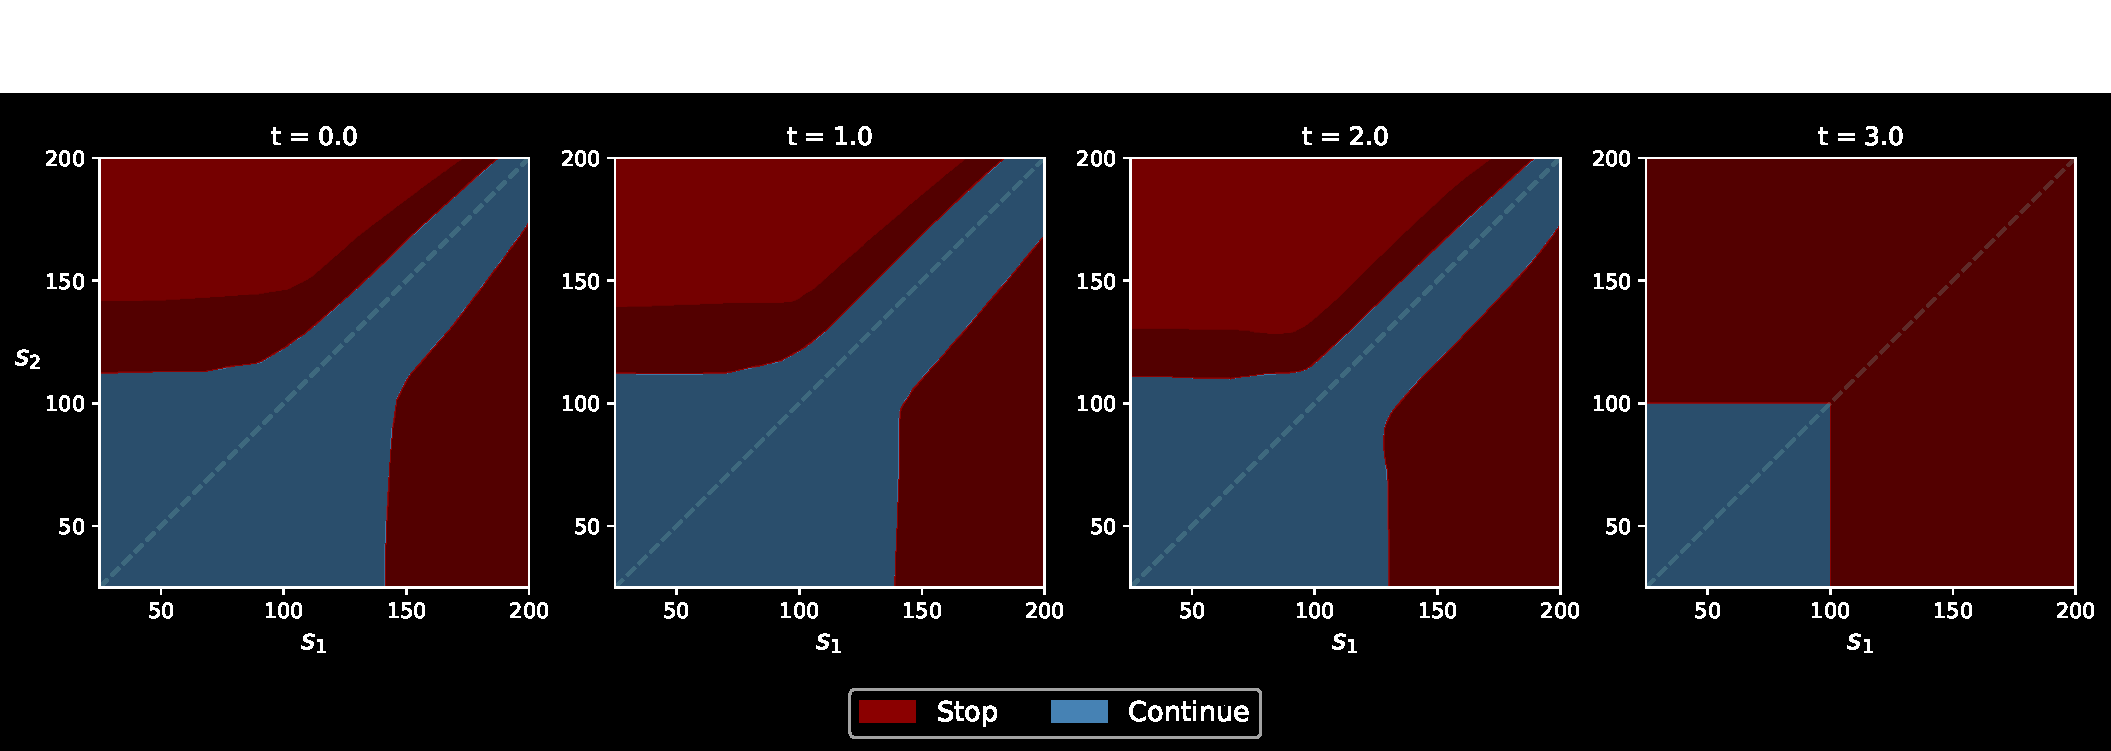
\includegraphics[scale = 0.42]{Figures/AsymCropped Max Call, d = 2, N = 9 (4 dates).pdf}
    \label{fig:asymCall}
    
    \scriptsize{
\textit{Note: The light red region is the reflection of $\calS_t^{(1)} = \calS_t \cap \ \{s_1 \ge s_2\}$ through the diagonal. %, i.e. $\varsigma(\calS_t^{(1)})$.
}} %This is to  illustrate that $\varsigma(\calS_t^{(1)}) \subseteq \calS_t^{(2)}$.  }}
\end{figure}


%\subsection{Spread Option}
%\subsection{Floating Strike Asian Option} \label{sec:Asian}
\subsection{American Lookback Call Option} \label{sec:Lkbk}


%Floating Strike Lookback Put Option
In the Black-Scholes world, consider an  American lookback option (\cref{ex:lookback}) with payoff $\Phi(\SSS_t) = (\max_{u\in[0,t]} S_u - K)^+$. In other words, it is a fixed strike lookback call of American type.  %$\Phi(\SSS_t) = (\gamma \max_{u\in[0,t]} S_u - S_t)^+$,
 As the running minimum is not needed, we can take $X_t = (S_t,Y_t)$, $Y_t = \max_{u\in[0,t]} S_u$ (hence $\calX = \{x=(s,y) \in \R_+^2 \ | \ s \le y\}$) and $\eta=1$, $\alpha(x) = y$, $\beta(x) = 0$ as in \cref{tab:lkbk}.    The ratio $\Xi(x) = \frac{s}{y}\in [0,1]$  is fed into the neural network. Notice that $1-\Xi(x) = \frac{y-s}{y}$ is the relative drawdown of the stock. 
We employ the parameters 
$$ T=1/2 \text{ ($6$ months)}, \quad  r=2\%, \quad \delta =4\%, \quad  \sigma = 30 \%.$$ 
These values are taken from  \citet{DaiKwok}, where the authors investigate analytical and geometric properties of the American lookback options. In particular, we aim at visualizing the stopping region in the $(s,y)$ plane, similar to Fig. $3$ in \cite{DaiKwok}.   %where the authors use a finite difference scheme to compute the initial price. 

To approximate the American price, we use a regular partition  with $N=200$ exercise opportunities prior to maturity. % giving  $\calT_{\!N} = \{\frac{n}{2N} \ | \ n=0,\ldots,N\}$. 
Moreover, we employ an even thinner  partition $\Pi_{N'}$, $N'=4 N = 800$ to obtain accurate estimates of  the running maximum. Due to the lookback feature,  taking $N \ll N'$ has little effect on the reward. Indeed, if the maximum up to time $t_n\in \Pi_{N}$  is attained at $t_m' \in [t_{n-1},t_{n}]$,  $t_m'\in \Pi_{N'},$ then $\varphi(X_{t_n})=\varphi(X_{t'_m})$ so the loss arising from exercising at $t_n$ instead of $t_m'$ is only due to the time value of money. 
After several experiments, we decided not to use importance sampling as it led to worse results.\footnote{Intuitively, a positive drift  increases the probability of exceeding the threshold, but at the same time the ratio $\frac{s}{y}$ is typically closer to $1$ and  favors continuation. On the flip side, a negative drift tends to increase the relative drawdown $\frac{y-s}{y}$ and in turn the odds of being in the stopping region, but the running maximum (hence the payoff) is reduced as well.} %with $\lambda = \frac{r-\delta}{\sigma}$
%only differs by the time decay $e^{-r(t_n - t'_{m})} \approx -\frac{rT}{N}$. %is only due to the time value of money.  %relative difference is only given by the time value of money, that is 
%}
%$\frac{D_{0,t'_{m}}\varphi(X_{t_m'})-D_{0,t_{n}}\varphi(X_{t_n})}{D_{0,t'_{m}}\varphi(X_{t_m'})} = 1-e^{-r(t_n - t'_{m})}  \approx \frac{1}{N}$.   


\begin{table}[H]
  \centering
  \caption{American lookback call,  $K=100$, $T=6$M.
 }
 
 \vspace{-2mm}
 
  \begin{tabular}{ccccc}
 \hline \hline
    Average Price  & Highest Price & Runtime   & European Price & Upper Bound\\
  \hline  \hline 
  16.827   (0.008)  &  16.844 (0.007) & 216.7  &  16.809 & 16.979 \\
  \hline \\[-1em]
  \multicolumn{5}{c}{%
  \begin{minipage}{13cm}%
    \tiny \textit{First  column:  average  of ten experiments (standard deviation in brackets). Second column: highest price  among the realisations and its standard deviation in brackets.  Third column:  average runtime (in seconds) per experiment for the training phase.  Last column: upper bound given by the forward value of the European price. }%
  \end{minipage}%
}
\end{tabular}
\vspace{2mm}
% \begin{flushleft}
% \scriptsize{
% \textit{Notes:  }}
% \end{flushleft}
\label{tab:resultLkbk}
  \end{table}
  
\cref{tab:resultLkbk} summarizes the result for $s_0=K=100$. The European price, denoted by $v^{\text{European}}$ gives a lower bound on the American price. Although explicit formulae exist for European lookback options in the Black-Scholes model \cite{Conze}, the price has been computed with Monte Carlo and same  partition for $[0,T]$. Indeed, the closed-form formula may well dominate the American price as discretizing time makes the %resulting
running maximum  negatively biased. 
The  last  column is the  forward value of European price, i.e.  $\frac{1}{D_{0,T}}v^{\text{European}} = e^{rT}v^{\text{European}}$, which  gives an upper bound for the American price.\footnote{Indeed, $(Y_{T}-K)^{+}$ dominates  $D_{0,\tau}(Y_{\tau}-K)^{+}$ pathwise for all stopping time $\tau \in \vartheta([0,T])$. Hence, $ v(0,S_0) \le \E^{\Q}[(Y_{T}-K)^{+}] = \frac{1}{D_{0,T}}v^{\text{European}}$. See also \citet{Conze}. } Since here $e^{rT} \approx 1.01$, the American option only offers little premium over its European counterparts. This is nevertheless  fortunate from a performance perspective as it gives a tight interval in which the American price must lie (see, e.g., \cite{Conze}).  We indeed obtain prices that are within the bounds. %Furthermore, we LSMC

We display the stopping and continuation region in \cref{fig:lkbkCall}. Obtaining an overall accurate boundary turns out to be challenging. Indeed,  visiting all the pairs $(s,y) \in \calX$ is difficult, especially when $s \ll y$. To deal with this issue, we randomize $s_0\in \calX$ and set the initial running maximum to $y_0 = K \vee s_0$. As in Fig. $3$ in \cite{DaiKwok}, we observe a flat boundary when $s\ll K$. That is, the neural network correctly set $G(t,s/y;\theta)$ approximately equal to the strike when $s/y \ll 1$, i.e. when the relative drawdown is large.  %$\xi \ll 1$.  % as $X_t$ tend to revert towards (and reflect at) the diagonal $\{s=y\}$ when $S$ beats the maximum. 

\begin{figure}[H]
    \centering
    \caption{Stopping and continuation regions (lookback call, $K=100$, $T=6$M).}
    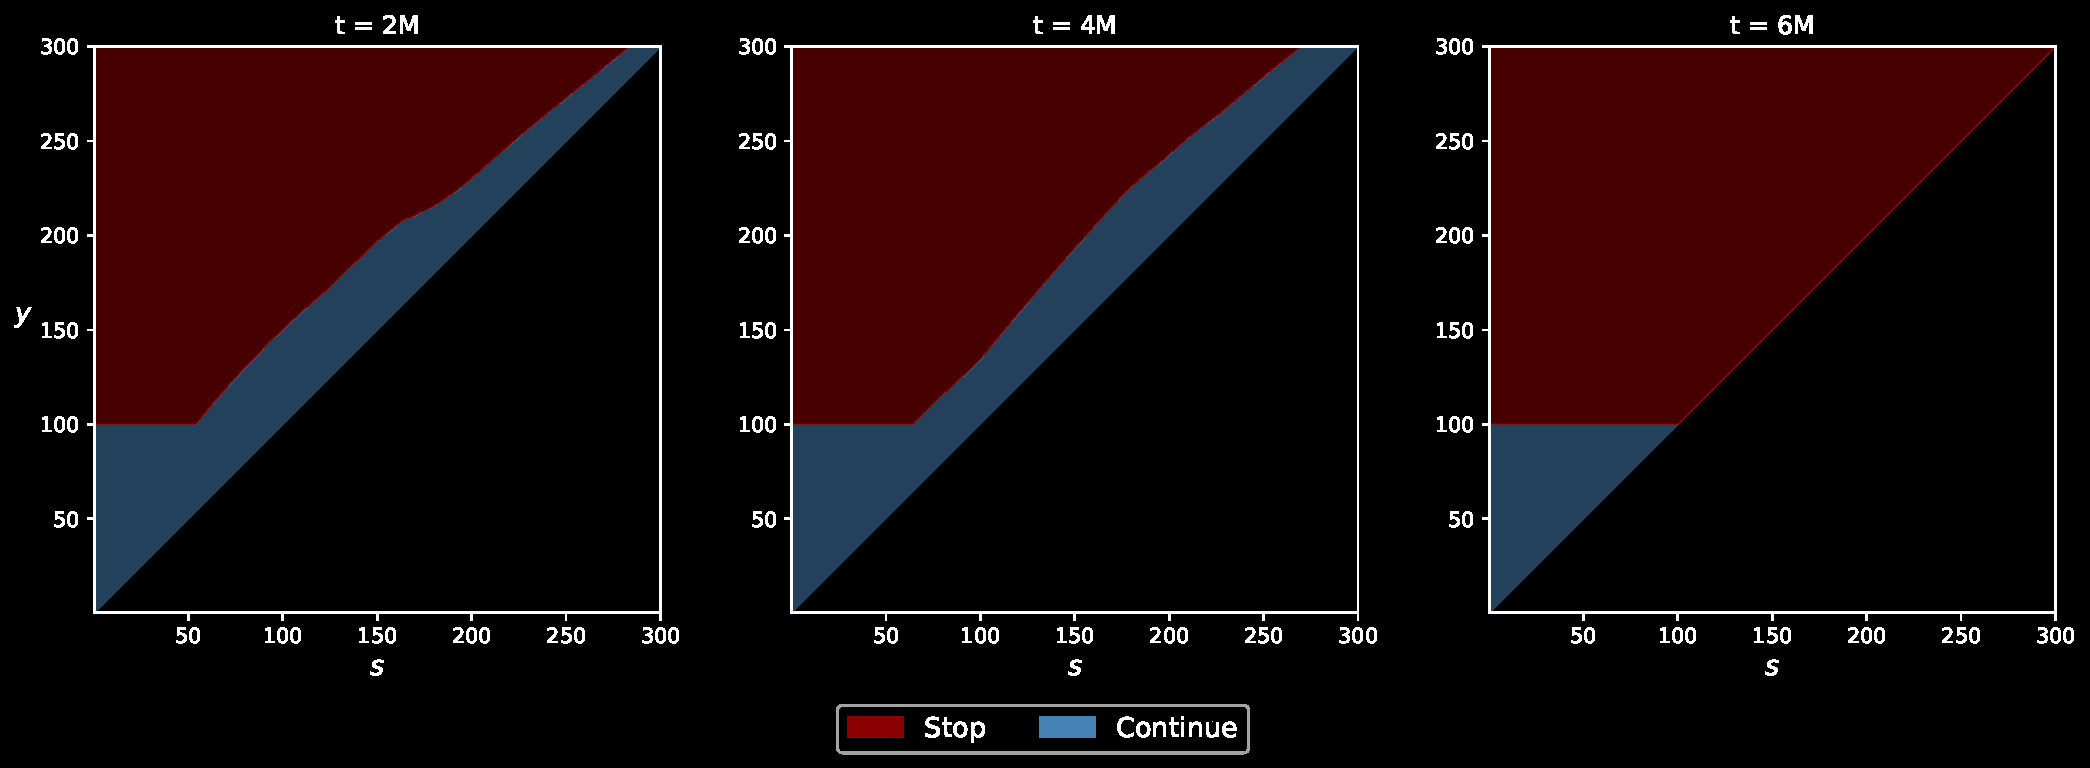
\includegraphics[scale = 0.42]{Figures/Best Lookback Call, d = 1, N = 126, lbda = -0.23, no rdm.pdf}
    \label{fig:lkbkCall}
    
    \scriptsize{
\textit{
}}
\end{figure}

